
\section{Introduction}

  Telecommunication in the HF Band using skywave propagation offers hundreds to thousands
  of kilometers coverage with relative low power and simple antennas, but it is also challenging,
  given the extreme limitation on throughtput  and very long transceiver turn-around times between tx and rx.

  HERMES is a digital telecommunication system for the HF band, which uses a high-performance HF modem and UUCP
  (Unix-to-Unix Communication Protocol), for email transport and other ad-hoc services.
  UUCP is arguably the most relevant store-and-forward system to date, in use since the late 70's
  for software exchange, email, bulletin board systems  news and even military communication. First released
  in Bell Labs' Unix Version 7, it is still present in all major Unixes (including Linux) and integrate seamless
  with email software like Postfix.

  Upper network layers are composed by email software infrastructure and Web Interface for management and access to the services.
  HERMES network topology is flexible, but tipically configured as star, with a ``gateway'' station located where Internet is available
  (in order to route data from stations located in isolated areas) and ``remote'' stations located at communities without access to
  other telecommunication systems.

%  While not a requirement at the time of development, UUCP lacks basic security and supports no encryption. HERMES,
%  on the other hand, is being used by indigenous communities in vulnerable contexts, in which encryption is a must-have.
%  While HERMES already provide some level of security, as individual messages can be encrypted, through the use of e-mail encryption,
%  all metadata is transported in clear, including the UUCP connection establishment and authentication procedures. This revised proposal
%  to NLNet involves adding security and encryption to UUCP, without the need for extra layers and extensive overhead (like using UUCP
%  over ssh over IP, which is not feasible in HF given the amount of tx/rx switches and huge overhead).

\section{HERMES Description}

This section briefly introduces what HERMES system can do today. HERMES is basically composed of:

\begin{itemize}
\item HF transceiver and associated antenna, connected to a computer;
\item Computer running the HERMES free software stack;
\item The computer provides local connectivity through WiFi (or other local-area network
  technology)
\end{itemize}

Rhizomatica developed the HERMES hardware which embedds all the needed parts for a simple to use
HF telecomunication equipment. Figure~\ref{fig1} and ~\ref{fig2} contains a picture of the HERMES box. The HERMES box contains
everything needed for joining a HERMES network, while users have access to the HERMES services over WiFi or ethernet.


\begin{figure}[h!]
  \centering
  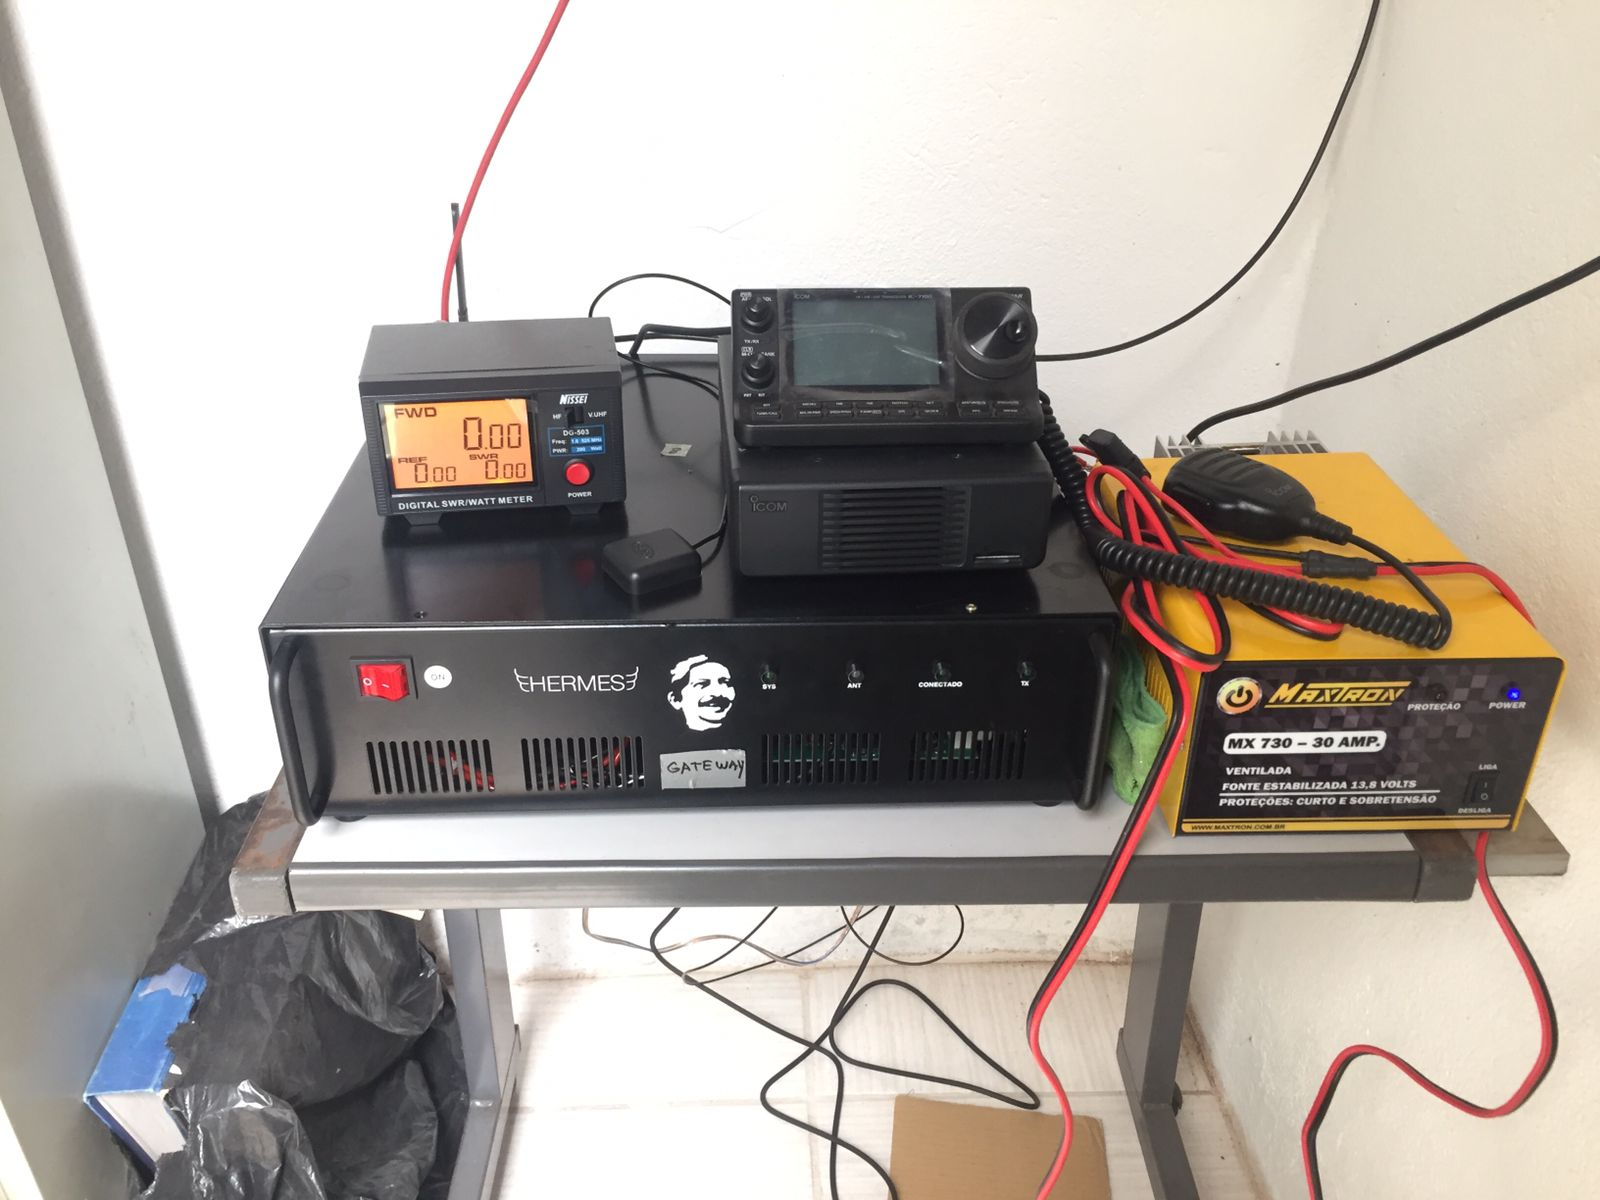
\includegraphics[scale=0.15]{hermes-pic1.jpeg}
  \caption{The HERMES hardware at a ``gateway'' location, a power supply (yellow), a standard HF voice radio (top right) and a wattmeter (top left).}
  \label{fig1}
\end{figure}

\begin{figure}[h!]
  \centering
  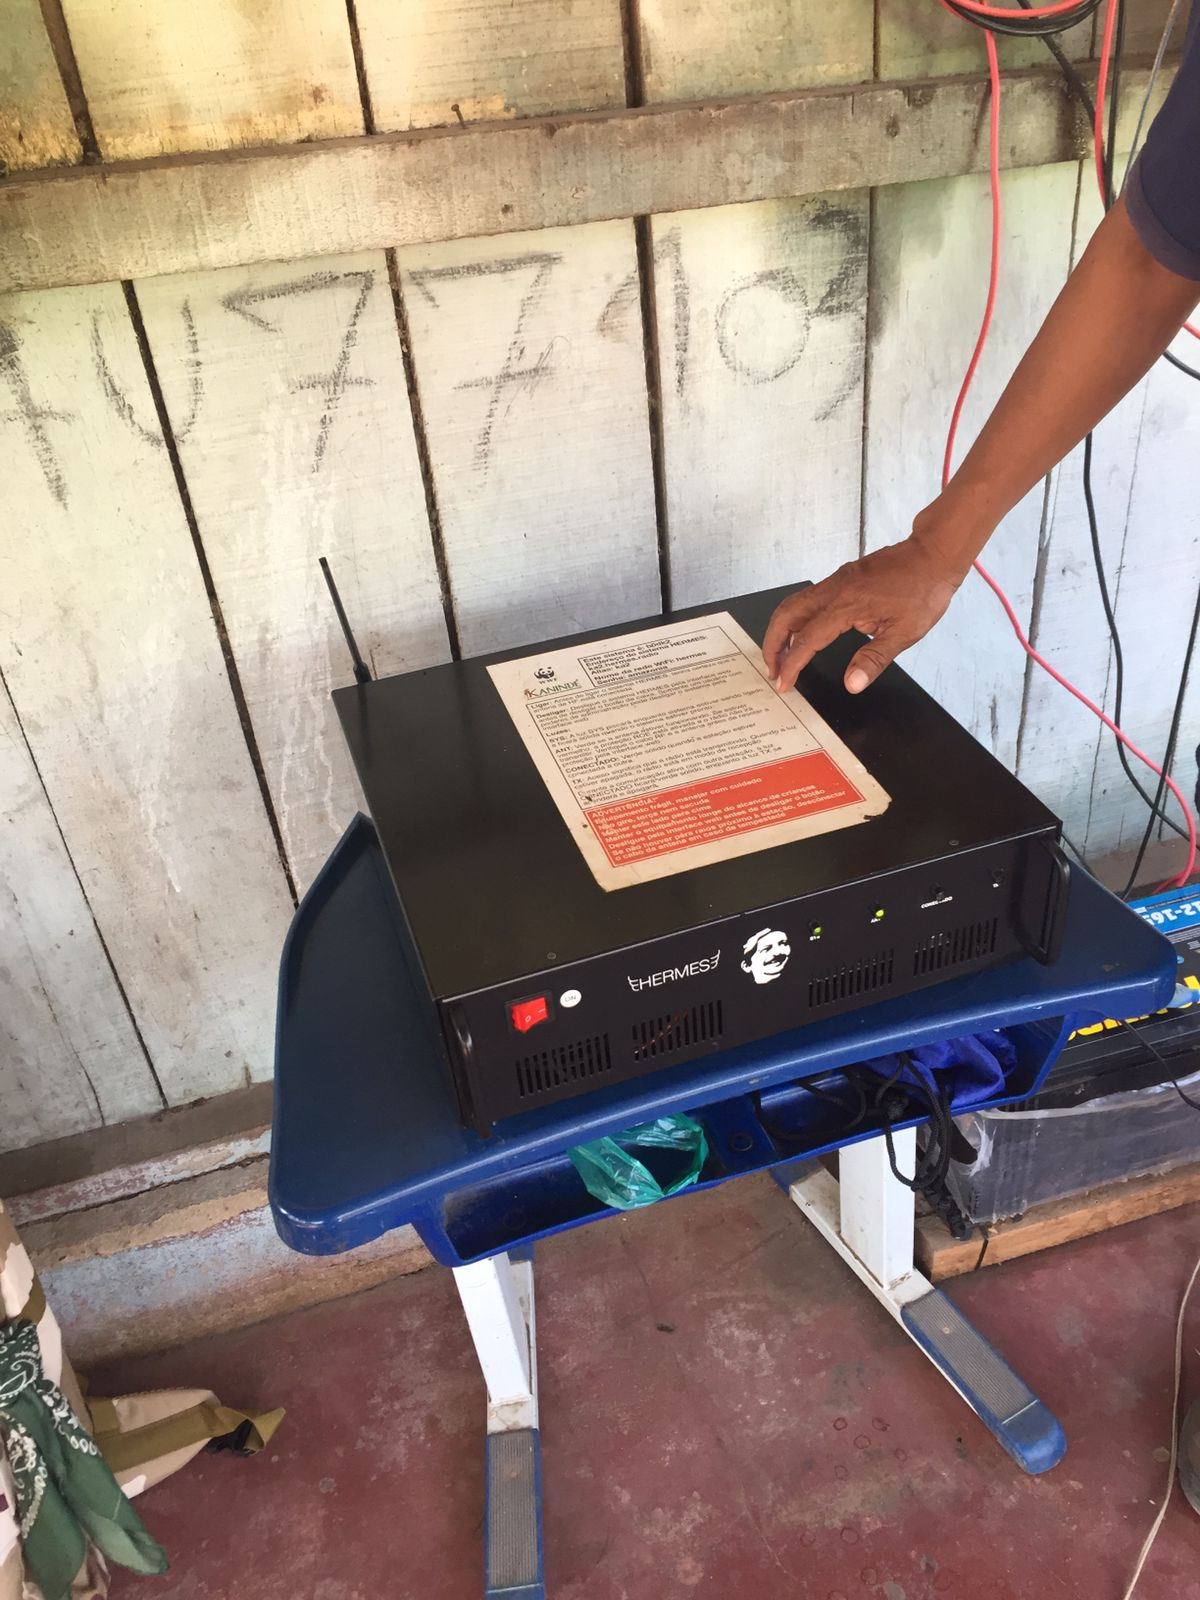
\includegraphics[scale=0.15]{hermes-pic2.jpeg}
  \caption{The HERMES hardware at a ``remote'' location, with a battery appearing the bottom left.}
  \label{fig2}
\end{figure}


HERMES uses GNU UUCP with Debian downstream patches (version 1.07-27 or greater, available at: \url{https://packages.debian.org/bullseye/uucp}).

Specific HERMES network stack source code, radio firmware and other system components are available at:

\begin{itemize}
\item Main network components and firmware: https://github.com/Rhizomatica/hermes-net
\item REST API: https://github.com/Rhizomatica/hermes-api
\item Web GUI: https://github.com/Rhizomatica/hermes-gui
\item Documentation: https://github.com/Rhizomatica/hermes-documentation
\end{itemize}

\section{HERMES System Architecture}
\label{sec:hermes-architecture}

This section provides an architecture-level description of HERMES as implemented by the software components referenced in
Section~\ref{sec:hermes-architecture-refs}. The focus is the HF data plane (store-and-forward payload transport over HF) and the
radio/modem control plane that makes that possible on commodity HF transceivers.

\subsection{Topology and station roles}

HERMES is commonly deployed as a star topology network with two roles:
\begin{itemize}
\item \textbf{Gateway station}: has Internet access and orchestrates synchronization with remote stations.
\item \textbf{Remote station}: provides local services (WiFi + web UI + email) and exchanges data with the gateway over HF.
\end{itemize}

Inter-station exchange is \textbf{asynchronous} (store-and-forward): payloads are queued locally and later transported over an HF link
during scheduled communication windows (often initiated by the gateway in round-robin fashion).

\subsection{Reference architecture (v2 / sBitx + VARA-compatible TNC + UUCP)}
\label{sec:hermes-architecture-reference}

The reference implementation described in this document corresponds to HERMES v2 (sBitx-based radio control) and a
\textbf{VARA-compatible TCP TNC interface} on localhost. In this model the station is composed of the following main processes:

\begin{itemize}
\item \textbf{Radio control daemon}: \verb|sbitx_controller| (from \verb|hermes-net/trx_v2-userland|), started by systemd as
  \verb|sbitx.service|. It controls RF hardware and exposes a shared-memory control/status interface used by other services.
\item \textbf{Modem/TNC}: either \textbf{VARA HF} (proprietary) or an \textbf{open modem} that implements the same VARA-style TCP TNC
  control/data sockets (e.g. \verb|hermes-modem|). The control socket is typically on TCP \verb|8300| and the data socket on
  \verb|8301| (base port + 1).
\item \textbf{UUCP transport}: GNU UUCP (\verb|uucico| + spool under \verb|/var/spool/uucp|), which provides store-and-forward job
  management and email transport integration.
\item \textbf{UUCP-to-modem bridge}: \verb|uucpd| (daemon) + \verb|uuport| (pipe helper) from \verb|hermes-net/uucpd|. This is the key
  component that turns the modem/TNC into an UUCP ``port''.
\item \textbf{Gateway orchestration (gateway-only)}: a scheduler such as \verb|caller.sh| (installed as \verb|caller.service|) that
  triggers \verb|uucico -S <station>| calls according to a schedule and station list.
\end{itemize}

\subsection{Station component diagram}

\begin{verbatim}
User devices (WiFi/LAN)
        |
      HTTP(S)
        v
 +--------------------+         +-----------------------+
 | Web UI / REST API  | <-----> | Mail stack (Postfix,  |
 | (external repos)   |         | Dovecot, etc)         |
 +--------------------+         +-----------+-----------+
                                             |
                                             v
                                     +-------+-------+
                                     | UUCP spool    |
                                     | /var/spool/uucp|
                                     +-------+-------+
                                             |
                                    uucico/uuport (per session)
                                             |
                               SysV SHM ring buffers (uucpd <-> uuport)
                                             |
                                             v
                                    +--------+--------+
                                    | uucpd (daemon)  |
                                    | VARA-style TNC   |
                                    +--------+--------+
                                             |
                 TCP control+data (8300/8301)|
                                             v
                                   +---------+---------+
                                   | Modem / TNC        |
                                   | (VARA or open)     |
                                   +---------+---------+
                                             |
                                   PTT ON/OFF + audio I/O
                                             |
                           SysV SHM control API (sbitx_controller)
                                             v
                                   +---------+---------+
                                   | sbitx_controller  |
                                   +-------------------+
\end{verbatim}

\subsection{Service orchestration (systemd)}

On Debian-based HERMES images these components are typically started by systemd. Reference unit files are shipped in
\verb|hermes-net/system_services/init/|. Some helper units for the Wine-based VARA modem are shipped by \verb|hermes-installer| under
\verb|hermes-installer/conf/x11vnc/|. The most relevant ones for the HF data plane are:

\begin{verbatim}
sbitx.service
  ExecStart=/usr/bin/sbitx_controller

# VARA HF (Wine + GUI): headless X server + VNC helper units
x11.service
  ExecStart=xvfb-run ... -n 69 -l xstartup

vnc.service
  ExecStart=x11vnc -display WAIT:69 ...

uucpd.service
  ExecStart=/usr/bin/uucpd -a 127.0.0.1 -p 8300 -r vara -o shm -f 2750p -m

caller.service   (gateway-only scheduler)
  ExecStart=/usr/bin/caller.sh

# Open modem (hermes-modem) alternative:
modem.service
  ExecStart=/usr/bin/mercury -v

uucpd-mercury.service   (typically installed as uucpd.service)
  ExecStart=/usr/bin/uucpd -a 127.0.0.1 -p 8300 -r vara -o shm
\end{verbatim}

\subsection{Interfaces: ports, paths and IPC}

The HERMES reference architecture uses a small set of explicit interfaces. The most important ones are summarized below.

\begin{table}[H]
\centering
\begin{tabularx}{\textwidth}{|l|l|X|}
\hline
\textbf{Layer} & \textbf{Interface} & \textbf{Notes} \\
\hline
Radio control & \verb|/etc/sbitx/core.ini|, \verb|/etc/sbitx/user.ini| & Installed by \verb|hermes-net|; defines radio IO, profiles, etc. \\
\hline
Radio control IPC & SysV SHM key \verb|66650| (\verb|controller_conn|) & Command/response API used by \verb|sbitx_client| and by \verb|uucpd| for PTT/LED/status. \\
\hline
Modem/TNC & TCP \verb|base_port| and \verb|base_port+1| (default 8300/8301) & VARA-style TNC interface: control socket (ASCII commands) + data socket (raw stream). \\
\hline
UUCP config & \verb|/etc/uucp/{config,sys,port,...}| & \verb|config| provides \verb|nodename|; \verb|sys| defines peers and schedules; \verb|port| uses \verb|type pipe|. \\
\hline
UUCP spool & \verb|/var/spool/uucp| & Store-and-forward queue; inspected with \verb|uustat| and logs with \verb|uulog|. \\
\hline
UUCP bridge IPC & SysV SHM keys \verb|66664|/\verb|66666|/\verb|66668| & Shared connector struct + in/out ring buffers used by \verb|uucpd| and \verb|uuport|. \\
\hline
\end{tabularx}
\end{table}

\subsection{Dynamic behavior (message and call flows)}

\subsubsection{Outbound session (gateway calls a remote station)}
\begin{enumerate}
\item Payloads (emails/messages/files) are queued locally and end up as UUCP jobs in the UUCP spool.
\item The gateway scheduler (e.g. \verb|caller.sh|) triggers an UUCP session: \verb|uucico -S <remote>|.
\item \verb|uucico| starts in master mode and invokes \verb|uuport| (configured as a \verb|type pipe| UUCP port).
\item \verb|uuport| attaches to \verb|uucpd|'s shared memory buffers and becomes \verb|uucico|'s byte-stream ``modem''.
\item \verb|uucpd| maintains a persistent TCP connection to the modem/TNC. When it sees outgoing bytes and is not connected, it issues a
  \verb|CONNECT <local> <remote>| command on the TNC control socket.
\item The modem/TNC drives the RF transmit/receive turn-taking and signals \verb|PTT ON|/\verb|PTT OFF| on the control socket. \verb|uucpd|
  translates these into actual radio keying (serial CAT or shared-memory keying via \verb|sbitx_controller|).
\item Once connected, bytes flow bidirectionally: \verb|uucico| $\leftrightarrow$ \verb|uuport| $\leftrightarrow$ \verb|uucpd| $\leftrightarrow$
  modem/TNC $\leftrightarrow$ HF RF link.
\end{enumerate}

\subsubsection{Inbound session (remote answers an incoming call)}
\begin{enumerate}
\item The modem/TNC is kept in listen mode by \verb|uucpd| (\verb|LISTEN ON|).
\item When a remote station calls in, the modem/TNC reports \verb|CONNECTED ...| on the control socket.
\item \verb|uucpd| detects this as an inbound connection and forks \verb|/usr/sbin/uucico| in slave mode, wiring its stdin/stdout to the same
  shared buffers used by \verb|uuport|.
\item The UUCP protocol runs and the spool is updated (receive jobs delivered; pending jobs may be sent back).
\end{enumerate}

\subsection{Variants}
\begin{itemize}
\item \textbf{Open modem (hermes-modem)}: provides a VARA-style TCP TNC interface, so from \verb|uucpd| perspective it behaves like VARA and
  uses the same integration path (control/data sockets, \verb|PTT ON/OFF| messages).
\item \textbf{ARDOP (legacy)}: supported by \verb|uucpd| using its \verb|-r ardop| mode; kept mainly for compatibility with older deployments.
\item \textbf{HERMES v1 (uBitx)}: legacy radio control uses \verb|ubitx_controller| and different service units (see \verb|hermes-net/system_services/init|).
\end{itemize}

\subsection{Architecture reference sources}
\label{sec:hermes-architecture-refs}

The architecture above is grounded in the following source trees and artifacts:
\begin{itemize}
\item \verb|hermes-net/uucpd| (bridge daemon \verb|uucpd| + port helper \verb|uuport| + modem integration code)
\item \verb|hermes-net/trx_v2-userland| (\verb|sbitx_controller| shared-memory control API)
\item \verb|hermes-net/system_services/init| (reference systemd unit files such as \verb|sbitx.service|, \verb|uucpd.service|, \verb|caller.service|)
\item \verb|hermes-modem| (open modem implementing VARA-style TCP TNC)
\end{itemize}


\section{HERMES Software Stack}

This section describes the main software components that implement the architecture described in
Section~\ref{sec:hermes-architecture-reference}.

HERMES deployments commonly use \textbf{VARA HF} as modem/TNC, but the system architecture is intentionally based on a
VARA-style TCP TNC interface, allowing \textbf{open modem} implementations (such as \verb|hermes-modem|) to be used as a drop-in
replacement. ARDOP is supported mostly for legacy compatibility.

For the network layer, UUCP is used. UUCP is a system for asynchronous
store-and-forward communication first released in Bell Labs Unix V7 in
the late 1970s, and still used today in niches, like communication over HF.

The \verb|uucpd| project (historically also referred to as \verb|uuardopd| / \verb|rhizo-uuardop| in older documents and code comments)
was developed to integrate UUCP with HF modems/TNCs.

At a high level, the HERMES station stack is made of:
\begin{itemize}
\item Radio control (\verb|sbitx_controller| and \verb|sbitx_client|)
\item Audio subsystem configuration (ALSA and related device plumbing)
\item Modem/TNC (VARA HF or open modem with VARA-style TCP interface)
\item UUCP (spool and \verb|uucico| sessions)
\item \verb|uucpd| bridge (\verb|uucpd| daemon + \verb|uuport| helper)
\item Upper services (web UI/API + email infrastructure)
\end{itemize}

\subsection{ALSA (Audio configuration)}

HERMES relies on a modem/TNC that exchanges baseband audio with the HF transceiver. On Linux, ALSA configuration is commonly used
to provide stable capture/playback device mapping for the modem process (including Wine-based VARA deployments).

The reference configuration shipped in \verb|hermes-net| is installed as \verb|/etc/asound.conf| from
\verb|hermes-net/system_services/alsa/asound-sbitx-hermes.conf|:
\begin{verbatim}
pcm.asymwine {
        type asym
        capture.pcm "hw:1,1"
        playback.pcm "hw:2,0"
}

pcm.!default {
        type plug
        slave.pcm "asymwine"
}

pcm.dsp {
        type plug
        slave.pcm "asymwine"
}
\end{verbatim}

The actual \verb|hw:X,Y| indices depend on your hardware. To identify them, use for example:
\begin{verbatim}
alsamixer
arecord -l
aplay -l
\end{verbatim}

\begin{figure}[h!]
  \centering
  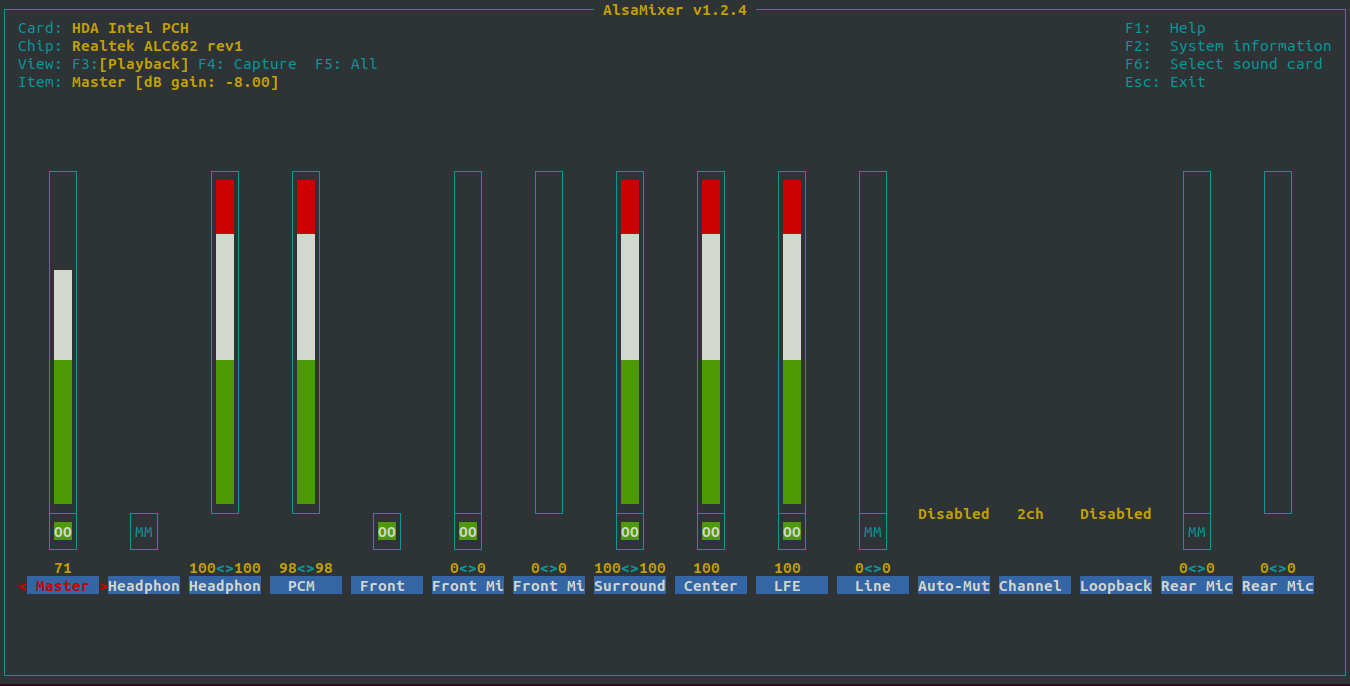
\includegraphics[scale=0.23]{screenshots/software_stack/alsamixer.png}
  \label{fig3}
\end{figure}

\subsection{Radio control: trx\_v2-userland (sbitx\_controller)}
\label{sec:trx-v2-userland}

HERMES v2 uses Rhizomatica's sBitx-based radio control stack from \verb|hermes-net/trx_v2-userland|. It builds two main executables:
\begin{itemize}
\item \verb|sbitx_controller|: a daemon that controls the radio (RF control + GPIO + I2C devices + audio DSP).
\item \verb|sbitx_client|: a CLI tool used for monitoring and setting radio parameters (frequency, mode, power, etc.).
\end{itemize}

\subsubsection{sbitx.service (systemd unit)}

The controller is typically started by systemd as \verb|sbitx.service|:
\begin{verbatim}
hermes-net/system_services/init/sbitx.service
  ExecStart=/usr/bin/sbitx_controller
\end{verbatim}

\subsubsection{Configuration files (/etc/sbitx)}

The default configuration files are expected at:
\begin{itemize}
\item \verb|/etc/sbitx/core.ini|
\item \verb|/etc/sbitx/user.ini|
\end{itemize}
They are installed by \verb|hermes-net| (\verb|make install|) from the \verb|trx_v2-userland/config/| directory.

\textbf{Core switches.} The most relevant toggles in \verb|core.ini| are:
\begin{itemize}
\item \verb|enable_shm_control = 1| (required for \verb|sbitx_client| and for \verb|uucpd -o shm| integration);
\item \verb|enable_websocket = 1| (optional; used by web GUIs for status streaming).
\end{itemize}

\subsubsection{Shared memory control API (sbitx\_client, uucpd)}

The controller exposes a System V shared memory segment (key \verb|66650|, type \verb|controller_conn|, see
\verb|hermes-net/include/sbitx_io.h|). This interface is used by \verb|sbitx_client| and also by \verb|uucpd| when configured with
\verb|-o shm|, allowing the modem/TNC integration to key PTT (and report status such as bitrate/SNR/bytes) without direct serial/CAT
access.

\subsubsection{Websocket status API (optional)}

When \verb|enable_websocket = 1|, \verb|sbitx_controller| starts an HTTPS/WSS server (Mongoose-based) that:
\begin{itemize}
\item listens on \verb|wss://0.0.0.0:8080|;
\item upgrades \verb|/websocket| to a websocket stream (JSON status updates);
\item serves static files from \verb|/etc/sbitx/web| (installed by \verb|hermes-net| from \verb|trx_v2-userland/web/|).
\end{itemize}
For example, the test page is typically available at \verb|https://<station>:8080/test.html| and connects to
\verb|wss://<station>:8080/websocket|.

TLS files are expected at:
\begin{itemize}
\item \verb|/etc/ssl/certs/hermes.radio.crt|
\item \verb|/etc/ssl/private/hermes.radio.key|
\end{itemize}

\subsubsection{Health checks}

\begin{verbatim}
systemctl status sbitx
sbitx_client -c get_frequency -p 0
sbitx_client -c get_mode -p 0

# If websocket is enabled:
ss -lntp | grep 8080
journalctl -f -u sbitx
\end{verbatim}

\subsection{Modem configuration}
\subsubsection{VARA}
VARA is a High Performance HF modem based on OFDM modulation.
VARA modem is the only piece of private software in the stack.\\
Currently, HERMES uses VARA HF 4.3 or newer as it's standard modem.
Use this protocol with your HERMES if you are looking for best performance available.\\

Please refer to the developer's website for download and instructions on installation and use: \\
\url{https://rosmodem.wordpress.com/}\\

\textbf{Configuration}\\
Edit /opt/VARA/VARA.ini.default to include your license key and callsign.

\textbf{Headless X/VNC services (Wine VARA).} In the reference Debian images, VARA HF is run under Wine and requires an X server. For
headless stations, \verb|hermes-installer| ships a minimal Xvfb + x11vnc setup:
\begin{verbatim}
hermes-installer/conf/x11vnc/x11.service
  ExecStart=xvfb-run --server-args="-screen 0 1024x768x24" ... -n 69 -l xstartup

hermes-installer/conf/x11vnc/vnc.service
  ExecStart=x11vnc -display WAIT:69 ...
\end{verbatim}
The \verb|xstartup| script (\verb|hermes-installer/conf/xstartup|) launches \verb|wine /opt/VARA/VARA.exe| (via \verb|xterm|) and starts
the window manager used by this session.

\textbf{Integration contract (VARA-style TCP TNC).} The rest of the HERMES HF stack does not interact with VARA through audio directly.
Instead, \verb|uucpd| connects to VARA's TCP interface (control socket on \verb|base_port|, data socket on \verb|base_port+1|; typically
\verb|8300|/\verb|8301|). VARA signals radio keying by sending \verb|PTT ON|/\verb|PTT OFF| on the control socket; \verb|uucpd| translates
that into actual PTT via serial or shared-memory radio control (\verb|-o shm| for sBitx).

\subsubsection{Open modem: hermes-modem (``mercury'' binary)}

Rhizomatica's open modem implementation is available at:
\url{https://github.com/Rhizomatica/hermes-modem/}

It provides a VARA-style TCP TNC interface (separate control and data sockets) so it can be used with the same \verb|uucpd| integration
path described above (\verb|uucpd -r vara ...|). In addition to ARQ links, it also provides a dedicated TCP port for broadcast data mode
(default \verb|8100|).

The \verb|hermes-modem| README documents its CLI options. In summary:
\begin{itemize}
\item \verb|-p| sets the ARQ TCP base port (control \verb|base|, data \verb|base+1|; default \verb|8300|).
\item \verb|-b| sets the broadcast TCP port (default \verb|8100|).
\item \verb|-x| selects the audio backend (\verb|alsa|, \verb|pulse|, \verb|shm|, etc.).
\end{itemize}

\textbf{Systemd unit (open modem).} A reference unit file is shipped as \verb|modem.service| (see
\verb|hermes-net/system_services/init/modem.service|). It starts the modem directly via \verb|/usr/bin/mercury| (installed from
\verb|hermes-modem| using \verb|make install|). On Linux, \verb|mercury| defaults to ALSA and uses the ALSA device \verb|default| for
capture/playback unless \verb|-i|/\verb|-o| are provided. When used, the corresponding \verb|uucpd-mercury.service| unit depends on
\verb|modem.service|.

\subsubsection{ARDOP}

ARDOP is a SDR(software defined radio) modem compatible with both HF and VHF radio transmissions. In HERMES it is mostly a legacy/optional
choice; the preferred integration target is the VARA-style TCP TNC interface described above.
The protocol can operate over a wide range of data rates by automatically adjusting for optimized performance under poor multi-path conditions.
Use this protocol with your HERMES if you are looking for a completely open-source and free option.

Download link: \url{https://github.com/DigitalHERMES/ardopc}\\

\textbf{Configuration}\\

The ardop binary should be in /usr/bin/ardop, which can be a
symbolic link to /usr/bin/{ardop1ofdm, ardop2, ardopofdm}.\\

ARDOP service file for the ICOM IC-7100 (USB connection, PTT done over serial):
\begin{verbatim}
[Unit]
Description=ARDOP daemon

[Service]
Type=simple
ExecStart=/usr/bin/ardop 8515 -c /dev/ttyUSB0 ARDOP ARDOP -k FEFE88E01C0001FD -u FEFE88E01C0000FD
ExecStop=/usr/bin/killall -s QUIT ardop
IgnoreSIGPIPE=no
#StandardOutput=null
#StandardError=null
StandardOutput=syslog
StandardError=syslog

[Install]
WantedBy=multi-user.target
\end{verbatim}

Service file when using a VOX based setup (eg. when using an interface like
the Signalink):
\begin{verbatim}
[Unit]
Description=ARDOP daemon

[Service]
Type=simple
ExecStart=/usr/bin/ardop 8515 ARDOP ARDOP
ExecStop=/usr/bin/killall -s QUIT ardop
IgnoreSIGPIPE=no
#StandardOutput=null
#StandardError=null
StandardOutput=syslog
StandardError=syslog

[Install]
WantedBy=multi-user.target
\end{verbatim}


\textbf{Start/stop ARDOP service:}
\begin{verbatim}
systemctl start ardop.service
systemctl stop ardop.service
\end{verbatim}


\textbf{See the log:}
\begin{verbatim}
journalctl -f -u ardop
\end{verbatim}

\subsubsection{Mercury (R\&D note)}
The name ``Mercury'' is used historically in HERMES for ongoing modem R\&D work. In practice, the current open modem implementation used in
HERMES deployments is \verb|hermes-modem| (previous subsection), which exposes the VARA-style TCP TNC interface expected by \verb|uucpd|.
The standalone Mercury R\&D repository (when applicable) is:
\url{https://github.com/Rhizomatica/mercury/}

\subsection{UUCP (Network configuration)}
UUCP is an acronym of Unix-to-Unix Copy.
It's a protocol for remote execution of commands and transfer of files, email and netnews between computers.

Since HERMES uses Debian GNU/Linux release Bullseye, UUCP packages are installed by default.

If you are not using Debian Bullseye, UUCP Debian package version 1.07-27 or higher should be used, for example,
the version from Debian Bullseye (11):
\url{https://packages.debian.org/bullseye/uucp}

UUCP command line examples follow. To copy a file to a remote host,
the following command adds a copy job to the uucp queue (``-r'' is used to
not start transmission after queuing):
\begin{verbatim}
uucp -C -r -d source.xxx AM4AAB\!/var/www/html/arquivos/${nodename}/
\end{verbatim}

Trigger the transmission of all queued jobs for host
AM4AAA:
\begin{verbatim}
uucico -S AM4AAA
\end{verbatim}

List the jobs:
\begin{verbatim}
uustat -a
\end{verbatim}

Kill a job:
\begin{verbatim}
uustat -k job
uustat -K
\end{verbatim}

See the log:
\begin{verbatim}
uulog
\end{verbatim}


\subsection{UUCPD: uucpd + uuport (UUCP to modem bridge)}
\label{sec:uucpd}

UUCPD is a set of tools that allow UUCP to operate over HF links by integrating \verb|uucico| with an HF modem/TNC. In the HERMES v2
reference architecture (Section~\ref{sec:hermes-architecture-reference}) the modem/TNC is accessed through a VARA-style TCP interface
(control socket on \verb|base_port|, data socket on \verb|base_port+1|).

The \verb|hermes-net/uucpd| package provides two executables:
\begin{itemize}
\item \verb|uucpd|: the always-on bridge daemon that keeps the modem/TNC in listen mode, initiates outgoing connects when data is available,
  and starts \verb|uucico| in slave mode when an inbound call is received.
\item \verb|uuport|: the helper invoked by \verb|uucico| when calling out (UUCP port \verb|type pipe|). It attaches to \verb|uucpd|'s shared
  memory buffers and provides a byte-stream interface to \verb|uucico|.
\end{itemize}

Communication between \verb|uuport| and \verb|uucpd| uses System V shared memory (connector struct + ring buffers). When configured with
\verb|uucpd -o shm|, radio keying/status is also done through the \verb|sbitx_controller| shared-memory interface (Section~\ref{sec:trx-v2-userland}).

Download link: \url{https://github.com/Rhizomatica/hermes-net/tree/main/uucpd} \\

\textbf{Install} \\
\\
To compile and install, type:
\begin{verbatim}
  $ make
  $ make install    
\end{verbatim}

\textbf{Configuration} \\
\\
Port configuration example at "/etc/uucp/port":
\begin{verbatim}
  port HFP
  type pipe
  command /usr/bin/uuport    
\end{verbatim}

An alternative Port configuration if you use a patched uucp ( for "\textbackslash Z" support, available in "improved-pipe.patch" which was added to uucp debian package version 1.07-27 ), where uuport passes the callsign of the station to be called to \verb|uucpd| with the uucp remote station name (allowing a single \verb|uucpd| instance to be used for different remote station callsigns):
\begin{verbatim}
  port HFP
  type pipe
  command /usr/bin/uuport -c \Z
\end{verbatim}

Sys protocol example (tested and works fine) at "/etc/uucp/sys":
\begin{verbatim}
  protocol y
  protocol-parameter y packet-size 512
  protocol-parameter y timeout 540
  chat-timeout 200
\end{verbatim}

Sys configuration example of remote system at "/etc/uucp/sys" (without login prompt):
\begin{verbatim}
  system remote
  call-login *
  call-password *
  time any
  port HFP
  chat "" \r
\end{verbatim}

Sys configuration example of remote system at "/etc/uucp/sys" (with login prompt - should call \verb|uucpd| with "-l"):
\begin{verbatim}
  system remote
  call-login *
  call-password *
  time any
  port HFP
  chat "" \r\c ogin: \L word: \P
\end{verbatim}

\textbf{Systemd service}

The reference systemd unit files shipped with \verb|hermes-net| include:
\begin{itemize}
\item \verb|hermes-net/system_services/init/sbitx.service|
\item \verb|hermes-net/system_services/init/uucpd.service|
\item \verb|hermes-net/system_services/init/caller.service| (gateway-only)
\end{itemize}

In the reference VARA deployment, the \verb|uucpd.service| ExecStart is:
\begin{verbatim}
ExecStart=/usr/bin/uucpd -a 127.0.0.1 -p 8300 -r vara -o shm -f 2750p -m
\end{verbatim}

\textbf{Start/stop uucpd service}
\begin{verbatim}
systemctl start uucpd.service
systemctl stop uucpd.service
\end{verbatim}

\textbf{Running uucpd (examples)}\\

Examples of \verb|uucpd| invocation:

\begin{verbatim}
$ uucpd -a 127.0.0.1 -c PU2BBB -p 8515 -t 60 -r ardop
$ uucpd -a 127.0.0.1 -p 8300 -r vara -o icom -s /dev/ttyUSB0 -f 2750p
$ uucpd -a 127.0.0.1 -p 8300 -r vara -o shm -f 2750p -m
\end{verbatim}


\textbf{See the log}
\begin{verbatim}
journalctl -f -u uucpd
\end{verbatim}

\textbf{uucpd usage}
\begin{verbatim}
 -c callsign:         Station Callsign (Eg: PU2HFF)
 -d remote_callsign:  Remote Station Callsign (optional)
 -r [ardop,vara]:     Choose modem/radio type
 -a tnc_ip_address:   IP address of the TNC
 -p tcp_base_port:    TCP base port of the TNC. ARDOP uses ports tcp_base_port and tcp_base_port+1
 -t timeout:          Time to wait before disconnect when idling (ARDOP ONLY)
 -f features:         Enable/Disable features.
     Supported features ARDOP: ofdm, noofdm (default: ofdm)
     Supported features VARA, BW mode: 500, 2300 or 2750 (default: 2300)
     Supported features VARA, P2P mode: "p" to enable (eg. 2300p)
 -s serial_device:    Set the serial device file path for keying the radio (VARA ONLY)
 -l:                  Tell UUCICO to ask login prompt (default: disabled)
 -F:                  Enable UUCP handshake fast-track (requires both ends; no-login chat)
 -m:                  Enable shared memory messaging parameter to uucp (requires patched uucp)
 -o [icom,ubitx,shm]: Sets radio type (supported: icom, ubitx or shm).
 -h:                  Prints this help
\end{verbatim}

\textbf{UUPORT Usage}
\begin{verbatim}
-c system_name:      Name of the remote system (default is don't change).
-e logfile.txt:      Log file (default is stderr).
-h:                  Prints this help
\end{verbatim}
\subsection{User Web Interface}

HERMES provides a web-based interface for sending messages, files and emails. It also allows for user management and radio configuration, among other features.
Current implementation also supports symmetric cryptography and audio/image compression.

The web app is composed of the front-end interface and a REST API.

\subsubsection{Hermes-GUI}
Hermes-GUI is the front-end interface built with Angular.js.

Source code is located at:
(\url{https://github.com/Rhizomatica/hermes-gui/}).\\

The project was generated with Angular CLI version 13.2.6.
Angular: 13.2.6 Angular CLI: 13.2.6 Node: 12.22.5 Package Manager: npm 8.5.2\\

\textbf{Requirements of the user interface:}

\begin{itemize}
\item ImageMagic: for image manipulation
\item VVC: Best free software low bitrate visual content compression codec: \url{https://github.com/fraunhoferhhi/}
% \item opusenc: para comprimir áudio
\item LPCNet: Best free software audio compression codec: \url{https://github.com/xiph/LPCNet}
\item GnuPG: For cryptography
\item hostapd: WiFi AP mode software
\end{itemize}

The Web interface can be accessed by typing any address in a browser
connected to the WiFi (set the DNS accordingly) or simply 10.0.0.1.\\


\textbf{Install node, npm}\\
Install node preferably(V12.22.5) and npm (node package manager) in your distro

Run 'npm install' inside the project path\\

\textbf{Development server}\\
Configure .env file with your parameters and run npx ts-node setEnv.ts to set .env values in enviroment.ts.

Run ng serve --configuration=en for a dev server in english, you can change the language to spanish (ng serve --configuration=es) or portuguese (ng serve --configuration=pt) if you wish. Navigate to http://localhost:4200/. The app will automatically reload if you change any of the source files.\\

\textbf{Code scaffolding}\\
Run ng generate component component-name to generate a new component. You can also use ng generate directive|pipe|service|class|guard|interface|enum|module.\\

%\textbf{Build & Publish}
%Access remotly machine in port 22 with ssh -p 22 hermes@[my_host_ip] type sudo su to admin verification Set origin main branch git checkout main Update project git pull Create an .env file like a .env.example in root directory Check and configure .env file with your parameters DEV/PROD and run npx ts-node setEnv.ts to set .env values in enviroment.ts. Remove all files in dist folder rm -r dist/ Run npm run build / ng build to build the project. The build artifacts will be stored in the dist directory. Copy them in /var/www/html/ directory cp -a dist/hermes/pt /var/www/html/ cp -a dist/hermes/es /var/www/html/ cp -a dist/hermes/en-US/ /var/www/html/ Done Navigate to HERMES

\textbf{Running unit tests}\\
Run ng test to execute the unit tests via Karma.\\

\textbf{Running end-to-end tests}\\
Run ng e2e to execute the end-to-end tests via Protractor.\\

\textbf{Further help}\\
To get more help on the Angular CLI use ng help or go check out the Angular CLI README.\\

\textbf{Interface Contents}\\
Inside the folder src you will find the angular templates for the system's interface.

On style.less there are the styling code, writen in less.

Inside the app folder, you will find the template components. The app-routing module.ts file is responsible for linking the templates to url adressess. and the app.component, the aplication root template.

For every system component, there will be a folder with the component.html, component.less, and component.ts. On the .html file there is the html angular template, and on the component.ts you will find typescript code related to that component.

Also inside the app folder, there is the \_services foder, where you can find common services shared between the components to access the [station-api] (https://github.com/DigitalHERMES/station-api).

On assets folder you find links to svgs and image files used on the interface design.

On the locale folder there are the xlf files for translation. For the translations, we are using i18n angular module. To generate translations, you need to use ng extract-i18n --output-path src/locale/ to generate the messages,xlf file and then xliffmerge --profile xliffmerge.json pt es to transpose the new data to both messages.es.xlf and messages.pt.xlf, where you can input the new tranlation tokens.

\subsubsection{Hermes-API}
Hermes-API is a REST api for use on Hermes stations to exchange messages between them.
It uses Lumen PHP Framework and composer to manage its own dependencies.\\

Source code is located at:
(\url{https://github.com/Rhizomatica/hermes-api/}).\\

\textbf{Server Requirements:}
\begin{itemize}
  \item Web server
  \item PHP >= 7.3
  \item OpenSSL PHP Extension
  \item PDO PHP Extension
  \item Mbstring PHP Extension
  \item SQLite DataBase\\
\end{itemize}

\textbf{Installation settings}\\

Setup your installation settings creating a .env file from .env.example\\

\textbf{Run Composer}\\

Composer is a dependency manager for PHP.

Run composer in your folder to install the dependencies and update relevant packages:
\begin{verbatim}
COMPOSER_ALLOW_SUPERUSER=1 composer install
COMPOSER_ALLOW_SUPERUSER=1 composer update

\end{verbatim}

\textbf{Copy hermes-api to /var/www/station-api/}\\

Go to your hermes-api folder and run:
\begin{verbatim}
  cp -rT . /var/www/station-api/
\end{verbatim}

\textbf{GNU Privacy Guard}\\

Create the folder for GNU Privacy Guard and change owner:
\begin{verbatim}
mkdir -p /var/www/.gnupg
chmod 700 /var/www/.gnupg
chown www-data:www-data /var/www/.gnupg
\end{verbatim}

\textbf{Setup public folders for UUCP}\\

Create and give permissions to inbox/outbox, downloads and temp folders to uucp public:
\begin{verbatim}
mkdir -p /var/www/station-api/storage/app/inbox
chmod 777 /var/www/station-api/storage/app/inbox
mkdir -p /var/www/station-api/storage/app/outbox
chmod 777 /var/www/station-api/storage/app/outbox
mkdir -p /var/www/station-api/storage/app/downloads
chmod 777 /var/www/station-api/storage/app/downloads
mkdir -p /var/www/station-api/storage/app/tmp
chmod 777 /var/www/station-api/storage/app/tmp
mkdir -p /var/www/station-api/storage/app/uploads
chmod 777 /var/www/station-api/storage/app/uploads
\end{verbatim}

The structure created is used by the app as follows:
/uploads (Files of outgoing messages)
/downloads (Files generated from the inbox received messages)
/inbox (incoming hermes message packs)
/outbox (hermes message pack for deliver)
/tmp (tmp files)\\

\textbf{Link folders}
\begin{verbatim}
ln -sf /var/www/station-api/public/ /var/www/html/api
\end{verbatim}

\textbf{Change owner of the app folder}
\begin{verbatim}
chown -R www-data:www-data /var/www/station-api/ 
\end{verbatim}

create database.sqlite file in database folder

To start a fresh database: php artisan migrate:refresh --seed\\

\textbf{Database setup}\\

Create a database named hermes and user with all privileges:

\begin{verbatim}
  echo "CREATE USER hermes IDENTIFIED BY 'db_hermes'; " > sql_commands.sql
  echo "CREATE DATABASE hermes;" >> sql_commands.sql
  echo "GRANT ALL PRIVILEGES ON hermes.* TO hermes;" >> sql_commands.sql
  
  mysql < sql_commands.sql
\end{verbatim}

Then go to your hermes-api folder and run Artisan for the migrations:
\begin{verbatim}
  cd /var/www/station-api/
  php artisan migrate
  php artisan db:seed    
\end{verbatim}

\textbf{Running on port 8000:}\\

> php -S localhost:8000 -t public\\

\textbf{Hermes Message Pack}\\
Hermes Message Pack is a tar gziped file named .hmp\\

% We use ``/var/www/html/arquivos'' as the default UUCP path to send
% files through the web interface.

%ps: WORK IN PROGRESS

%Email server (MTA) can either run locally or only in a central host with
%Internet. Stations can either opt to connect to a central station on demand,
%have some pre-defined schedule, or the central station connects to the
%community stations doing a pooling, delivering and downloading emails and
%files.

%\subsection{WebPhone}

%WORK IN PROGRESS

%\url{https://gitlab.tic-ac.org/keith/webphone/wikis/hermes}
